% Grossmont College -- Chem 141 Lab 1: Measuring Density with Different Types of Glassware
% Cameron Carroll
% February 2014


\documentclass[fleqn,titlepage]{article}

\renewcommand*\rmdefault{ppl}

\usepackage[version=3]{mhchem} % Package for chemical equation typesetting
\usepackage{tabu}
\usepackage{wasysym}
\usepackage{listings}
\usepackage{scrextend}
\lstset{language=Matlab}

% set 1" margins on 8.5" x 11" paper
% top left is measured from 1", 1"
\topmargin 0in
\oddsidemargin 0in
\evensidemargin 0in
\headheight 0in
\headsep 0in
\topskip 0in
\textheight 9in
\textwidth 6.5in

\usepackage{graphicx} % Required for the inclusion of images

\setlength\parindent{0pt} % Removes all indentation from paragraphs

\renewcommand{\labelenumi}{\alph{enumi}.} % Make numbering in the enumerate environment by letter rather than number (e.g. section 6)

%\usepackage{times} % Uncomment to use the Times New Roman font

%----------------------------------------------------------------------------------------
% DOCUMENT INFORMATION
%----------------------------------------------------------------------------------------

\begin{document}

\begin{titlepage}
  \mbox{}\\[1.25cm]
  \textbf{\LARGE Cameron Carroll \\ Grossmont College}\\[2.25cm]
  \begin{center}
    \textbf{\huge Experiment 1: \\ Measuring Density with Different Types of Glassware}\\[2.50cm]
  \end{center}
  \textbf{\LARGE Professor: Martin Larter \\ Chemistry 141-0692} \\
  \vfill
  \center{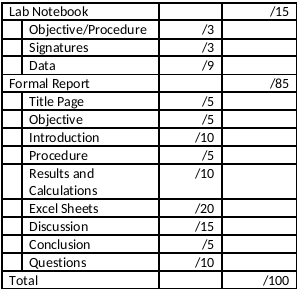
\includegraphics{./rubric_stdev}}
  \center{\textbf{\LARGE Performed --} {\LARGE January 30 and February 4, 2014}}
  \center{\textbf{\LARGE Submitted --} {\LARGE February 11, 2014}}
\end{titlepage}

%----------------------------------------------------------------------------------------
% SECTION 1
%----------------------------------------------------------------------------------------
\section*{Objective}
  \paragraph{} To introduce the analysis of uncertainty in experimental data. To calibrate a few pieces of common laboratory glassware and determine their overall accuracy and precision. To determine the density of Coke and Diet Coke and analyze post-calibration data uncertainty.

%----------------------------------------------------------------------------------------
% SECTION 2
%----------------------------------------------------------------------------------------
\section*{Introduction}
  \paragraph{} One of the most important parts of laboratory work is managing errors in the data. Unless care is taken, these errors can quickly snowball to nullify experimental efforts and conclusions. Error analysis can also indicate problems with the experiment: Either complete catastrophic failure or consistently bad technique.
  \paragraph{} There are two measures of error that we will consider: precision and accuracy. Precision is an indication of repeatability in measurement while accuracy shows how far from the true value our experimental value is. Further, there are three types of error: systematic, gross, and random. Systematic error is the one that indicates bad technique: precision may be fair, but accuracy is poor. (Values are offset in a particular direction.)
  Gross error indicates a serious, unrecoverable mistake. Finally, random error is an unavoidable consequence of the precision of instruments used.
  \paragraph{} We will use some basic statistical tools in this and later analyses. Among these are the percent error, used to find average distance from true value;
  \begin{center}$\text{percent error} = (100\%)
    \frac{\text{measured\ value} - \text{theoretical\ value}}{\text{theoretical\ value}}$\end{center}
  Arithmetic mean, which measures the common average...
  \begin{center}$\text{mean}=\frac{1}{n}\sum\limits_{i=1}^n a_i$\end{center} where $n$ is the number of elements and $a_i$ is the current element;
  The median, which denotes the middle value in the set. (The probability that any value of the set is larger or smaller is 1/2.)
  \begin{center}$P(X \le m) \ge 0.5$ and $P(X \ge m) \ge 0.5$\end{center} where X is any datum and m is the median;
  The spread, which represents scattering in the data. The simplest and probably least effective measure of spread is the range, which is simply the difference between the largest and smallest elements;
  \begin{center}$\text{range} = \text{largest datum} - \text{smallest datum}$\end{center}
  The deviation, or distance from the average,
  \begin{center} $\text{deviation} = |\overline{X} - X_i|$\end{center} where $\overline{X}$ is the average and $X_i$ is any datum;
  And finally standard deviation, which is a measure of precision quantifying how the data in general are offset relative to the average. 
 \begin{center}$\text{standard deviation} = \sigma = 
  \sqrt{\frac{\Sigma (x-\bar{x})^2}{n-1}}$\end{center}
  Standard deviation is used rather than significant figures to determine precision because technique plays a large part in the uncertainty of the measurement, which significant figures fail to capture.
  \paragraph{} This experiment involves performing a series of repeated measurements using three different types of glassware, which gives an idea of the precision of each after application of the aforementioned statistical tools.
  Furthermore, we know what the true values should be allowing us to get an idea of the accuracy of each piece of glassware.

%----------------------------------------------------------------------------------------
% SECTION 3
%----------------------------------------------------------------------------------------
\newpage
\section*{Procedure}
\begin{itemize}
  \item  \textbf{Part A:} \\
    \begin{addmargin}[1em]{1em}
      Lehman, J. (Et alia), `Measuring Density with Different Types of Glassware' \\
      Grossmont College, Chemistry 141 Lab Manual, 6th edition, pp 1-13 \\
      El Cajon, California
    \end{addmargin}
  \item \textbf{Part B:}
    \paragraph{} The procedure for part B was undefined and left to choice. I essentially duplicated the pipet calibration procedure from part A.
    \begin{enumerate}
      \item Cleaned a 10 mL pipet and rinsed with some of the sample (either Coke or Diet Coke)
      \item Washed and weighed empty bottle 
      \item Used the pipet to deliver aliquots of sample to the bottle, recording the new mass after each aliquot.
      \item (Repeated procedure for the other variety of pop.)
    \end{enumerate}
\end{itemize}

%----------------------------------------------------------------------------------------
% SECTION 4
%----------------------------------------------------------------------------------------
\section*{Results \& Calculations}
  \subsection*{Beaker Calibration}
    \begin{center}
      \begin{tabu}{|c|c|c|c|}
        \hline
        Trial & 1 & 2 & 3 \\
        \hline
        Mass of Beaker (full) & 96.601g & 96.509g & 96.398g \\
        Mass of Beaker (emptied) & 48.227g & 48.224g & 48.032g \\
        Mass of \ce{H2O} Delivered & 48.374g & 48.285g & 48.366g \\
        \hline
        Temperature & \multicolumn{3}{c|}{$23.5\,^{\circ}\mathrm{C}$} \\
        Density of \ce{H2O} & \multicolumn{3}{c|}{0.997418 $\frac{\text{g}}{\text{mL}}$} \\
        Average Mass Delivered & \multicolumn{3}{c|}{48.342g} \\
        `True' Volume Delivered & \multicolumn{3}{c|}{48.342mL} \\
        Standard Deviation & \multicolumn{3}{c|}{0.0492g} \\
        Relative Standard Deviation & \multicolumn{3}{c|}{0.102\%} \\
        Percent Error & \multicolumn{3}{c|}{3.32\%} \\
        68\% of Values Between & \multicolumn{3}{c|}{48.292 and 48.391g} \\
        95\% of Values Between & \multicolumn{3}{c|}{48.243 and 48.440g} \\
        99\% of Values Between & \multicolumn{3}{c|}{48.194 and 48.489g} \\
        \hline
      \end{tabu}
    \end{center}

  \subsection*{Graduated Cylinder Calibration}
    \begin{center}
      \begin{tabular}{|c|c|c|c|c|c|c|}
        \hline
        Trial & 1 & 2 & 3 & 4 & 5 & 6 \\
        \hline
        Mass of Bottle (after delivery) & 36.179g & 46.006g & 55.932g & 65.801g & 75.369g & 85.219g \\
        Mass of Bottle (tare) & 26.429g & 36.179g & 46.006g & 55.932g & 65.801g & 75.369g \\
        Mass of \ce{H2O} Delivered & 9.750g & 9.827g & 9.926g & 9.869g & 9.568g & 9.850g \\
        \hline
        Temperature & \multicolumn{6}{c|}{$23.5\,^{\circ}\mathrm{C}$} \\
        Density of \ce{H2O} & \multicolumn{6}{c|}{0.997418 $\frac{\text{g}}{\text{mL}}$} \\
        Average Mass Delivered & \multicolumn{6}{c|}{9.798g} \\
        Standard Deviation & \multicolumn{6}{c|}{0.127g} \\
        Relative Standard Deviation & \multicolumn{6}{c|}{1.296\%} \\
        `True' Volume Delivered & \multicolumn{6}{c|}{$9.823 \pm 0.127$mL} \\
        Percent Error & \multicolumn{6}{c|}{1.77\%} \\
        68\% of Values Between & \multicolumn{6}{c|}{9.671 and 9.925g} \\
        95\% of Values Between & \multicolumn{6}{c|}{9.544 and 10.052g} \\
        99\% of Values Between & \multicolumn{6}{c|}{9.417 and 10.179g} \\
        \hline
      \end{tabular}
    \end{center}

  \subsection*{Pipet Calibration}
    \begin{center}
      \begin{tabular}{|c|c|c|c|c|}
        \hline
        Trial & 1 & 2 & 3 & 4 \\
        \hline
        Mass of Bottle (after delivery) & 36.402g & 46.298g & 56.079g & 66.145g \\
        Mass of Bottle (tare) & 26.452g & 36.402g & 46.298g & 56.079g  \\
        Mass of \ce{H2O} Delivered & 9.950g & 9.896g & 9.781g & 10.066g \\
        \hline
        Temperature & \multicolumn{4}{c|}{$23.5\,^{\circ}\mathrm{C}$} \\
        Density of \ce{H2O} & \multicolumn{4}{c|}{0.997418 $\frac{\text{g}}{\text{mL}}$} \\
        Average Mass Delivered & \multicolumn{4}{c|}{9.923g} \\
        Standard Deviation & \multicolumn{4}{c|}{0.118g} \\
        Relative Standard Deviation & \multicolumn{4}{c|}{1.189\%} \\
        `True' Volume Delivered & \multicolumn{4}{c|}{$9.949 \pm 0.118$mL} \\
        Percent Error & \multicolumn{4}{c|}{0.51\%} \\
        68\% of Values Between & \multicolumn{4}{c|}{9.805 and 10.042g} \\
        95\% of Values Between & \multicolumn{4}{c|}{9.686 and 10.160g} \\
        99\% of Values Between & \multicolumn{4}{c|}{9.568 and 10.278g} \\
        \hline
      \end{tabular}
    \end{center}

  \subsection*{Density of Coke}
    \begin{center}
      \begin{tabular}{|c|c|c|c|c|c|}
        \hline
        Trial & 1 & 2 & 3 & 4 & 5 \\
        \hline
        Volume Delivered & 9.949g & 9.949g & 9.949g & 9.949g & 9.949g \\
        Mass Delivered & 10.296g & 10.330g & 10.326g & 10.340g & 10.314g  \\
        Density & 1.0349$\frac{\text{g}}{\text{mL}}$ & 1.0383$\frac{\text{g}}{\text{mL}}$ & 1.0379$\frac{\text{g}}{\text{mL}}$ & 1.0393$\frac{\text{g}}{\text{mL}}$ & 1.0367$\frac{\text{g}}{\text{mL}}$  \\
        \hline
        Temperature & \multicolumn{5}{c|}{$23.8\,^{\circ}\mathrm{C}$} \\
        Average Density & \multicolumn{5}{c|}{1.0374$\frac{\text{g}}{\text{mL}}$} \\
        True Density & \multicolumn{5}{c|}{1.0420$\frac{\text{g}}{\text{mL}}$} \\
        Standard Deviation & \multicolumn{5}{c|}{0.00170$\frac{\text{g}}{\text{mL}}$} \\
        Relative Standard Deviation & \multicolumn{5}{c|}{0.164\%} \\
        Percent Error & \multicolumn{5}{c|}{0.441\%} \\
        68\% of Values Between & \multicolumn{5}{c|}{1.0357 and 1.0391$\frac{\text{g}}{\text{mL}}$} \\
        95\% of Values Between & \multicolumn{5}{c|}{1.0340 and 1.0408$\frac{\text{g}}{\text{mL}}$} \\
        99\% of Values Between & \multicolumn{5}{c|}{1.0323 and 1.0425$\frac{\text{g}}{\text{mL}}$} \\
        \hline
      \end{tabular}
    \end{center}

  \subsection*{Density of Diet Coke}
    \begin{center}
      \begin{tabular}{|c|c|c|c|c|c|}
        \hline
        Trial & 1 & 2 & 3 & 4 & 5 \\
        \hline
        Volume Delivered & 9.949g & 9.949g & 9.949g & 9.949g & 9.949g \\
        Mass Delivered & 9.919g & 9.976g & 9.744g & 9.969 & 9.927g  \\
        Density & 0.997$\frac{\text{g}}{\text{mL}}$ & 1.00271$\frac{\text{g}}{\text{mL}}$ & 0.979$\frac{\text{g}}{\text{mL}}$ & 1.00201$\frac{\text{g}}{\text{mL}}$ & 0.998$\frac{\text{g}}{\text{mL}}$  \\
        \hline
        Temperature & \multicolumn{5}{c|}{$23.8\,^{\circ}\mathrm{C}$} \\
        Average Density & \multicolumn{5}{c|}{0.996$\frac{\text{g}}{\text{mL}}$} \\
        True Density & \multicolumn{5}{c|}{0.997$\frac{\text{g}}{\text{mL}}$} \\
        Standard Deviation & \multicolumn{5}{c|}{0.00950$\frac{\text{g}}{\text{mL}}$} \\
        Relative Standard Deviation & \multicolumn{5}{c|}{0.954\%} \\
        Percent Error & \multicolumn{5}{c|}{0.100\%} \\
        68\% of Values Between & \multicolumn{5}{c|}{0.987 and 1.00550$\frac{\text{g}}{\text{mL}}$} \\
        95\% of Values Between & \multicolumn{5}{c|}{0.977 and 1.0150$\frac{\text{g}}{\text{mL}}$} \\
        99\% of Values Between & \multicolumn{5}{c|}{0.968 and 1.0245$\frac{\text{g}}{\text{mL}}$} \\
        \hline
      \end{tabular}
    \end{center}

  \subsection*{Calculations}
    \subsubsection*{Mass Delivered}
      \begin{center}$M_{\text{delivered}} = M_{\text{after delivery}} - M_{\text{empty or tare}}$\end{center}
      \begin{center}$9.950\text{g} = 36.402 - 26.452\text{g}$\end{center}

    \subsubsection*{Average Mass Delivered}
      \begin{center}$\overline{M} = \frac{\sum\limits_{i}^{n}M_{i}}{n}$\end{center}
      \begin{center}$9.923\text{g} = \frac{9.950 + 9.896 + 9.781 + 10.066\text{g}}{4}$\end{center}

    \subsubsection*{Deviation from Average}
      \begin{center}$d = |\overline{M} - M_i|$\end{center}
      \begin{center}$0.027\text{g} = |9.923 - 9.950\text{g}|$\end{center}

    \subsubsection*{Standard Deviation}
      \begin{center}$\sigma = \sqrt{\frac{\sum\limits_{i}^{n}(d_{i})^2}{n-1}}$\end{center}
      \begin{center}$0.118\text{g} = \sqrt{\frac{(0.027)^2 + (0.027)^2 + (0.142)^2 + (0.143)^2\text{g}}{3}}$\end{center}

    \subsubsection*{Confidence Intervals}
      \begin{center}$\text{[68\%, 95\%, 99\%] confidence interval} = \overline{M} \pm \text{[1, 2, 3]} * \sigma$\end{center}
      \begin{center}$68\% = 9.805 \text{ to } 10.041\text{g} = (9.923 - 1*0.118) \text{ to } (9.923 + 1*0.118)\text{g}$\end{center}
      \begin{center}$95\% = 9.687 \text{ to } 10.159\text{g} = (9.923 - 2*0.118) \text{ to } (9.923 + 2*0.118)\text{g}$\end{center}
      \begin{center}$99\% = 9.569 \text{ to } 10.277\text{g} = (9.923 - 3*0.118) \text{ to } (9.923 + 3*0.118)\text{g}$\end{center}

    \subsubsection*{Density}
      \begin{center}$\rho = \frac{\text{mass}}{\text{volume}}$\end{center}
      \begin{center}$\text{volume delivered} = \frac{\text{average mass delivered}}{\rho}$\end{center}
      \begin{center}$48.342\text{mL} = \frac{48.342\text{g}}{1.00 \frac{\text{g}}{\text{mL}}}$\end{center} 

%----------------------------------------------------------------------------------------
% SECTION 5
%----------------------------------------------------------------------------------------
\section*{Discussion}
  \subsection*{Part A}
    \paragraph{} The accuracy calculations show that some pieces of glassware are simply more accurate than the others. Working out the precision, however, points to some systematic error in all cases.

    \paragraph{} Looking at the former, it's pretty clear that the pipet is the most accurate and the beaker the least so...
    \center{$\%\text{E}_\text{beaker} > \%\text{E}_\text{graduated\ cylinder} > \%\text{E}_\text{pipet} = 3.32\% > 1.77\% > 0.51\% $} \\[0.2cm]
    which is the expected result. Note that despite having $\frac{1}{5}$ of the volume, the graduated cylinder has half the percent error of the beaker. Also note that except for one datum in the pipet calibration section, \emph{all} data is short of the expected delivery value. I believe that the source of this error is incorrect reading of the meniscus -- Until asking for clarification during pipet calibration, I had been using inconsistent points of the meniscus. Because the readings are supposed to be from the very bottom of the meniscus bowl, and because this is the last possible reading without parallax error, every other reading should be below the intended delivery value.

    \paragraph{} The precision values are somewhat misleading, which I argue is from the combined effort of a fluke and bad technique. The relative standard deviation for the beaker measurements is unexpectedly low... \\
    \center{$\%\text{RSD}_{graduated\ cylinder} > \%\text{RSD}_{pipet} > \%\text{RSD}_{beaker} = 1.296\% > 1.189\% > 0.102\%$} \\[0.2cm]
    I believe there are a couple of reasons for which the beaker RSD is so low: First of all, there are very few measurements so luck could easily have swayed this value. Also, the main issue with the graduated cylinder and pipet data was my technique reading the meniscus, which is much easier on a graduated cylinder where the meniscus is very wide and relatively flat. \\
    As expected, however, the pipet has a lower standard deviation than the graduated cylinder.

    \paragraph{} Comparing standard deviations to the published uncertainties for each piece of glassware gives another indication of poor technique with the pipet and that the beaker was a statistical fluke. The graduated cylinder, on the other hand, lies fairly close to its published uncertainty. \\
    \center{$\text{uncertainty}_\text{beaker} > \text{standard\ deviation}_\text{beaker} = 5 > 0.0492\text{mL}$}
    \center{$\text{uncertainty}_\text{graduated\ cylinder} \approx \text{standard\ deviation}_\text{graduated\ cylinder} = 0.1 \approx 0.127\text{mL}$}
    \center{$\text{uncertainty}_\text{pipet} < \text{standard\ deviation}_\text{pipet} = 0.02 < 0.118\text{mL}$}

    \paragraph{} From my data, the pipet is more accurate than the graduated cylinder which is more accurate than the beaker. The data shows the pipet to be more precise than the graduated cylinder but much less precise than its significant figure uncertainty. It also shows the beaker to be the most precise by far, which is deemed a statistical fluke and thus an unreliable conclusion.

  \subsection*{Part B}
    \paragraph{} I decided to use a pipet based on my data from part A; It provided the best results for accuracy even with my relatively poor technique. After adding in calibrated offset (using 9.949mL delivery volume, or the average from pipet calibration) the standard deviation values were on the order of the significant figure uncertainty.

    \paragraph{} The calculated densities were very close to their true values, yielding low percent errors and high accuracy. \\
    \center{$\text{true\ density}_{coke} \approx \text{average\ density}_{coke} = 1.0374 \approx 1.0420\frac{\text{g}}{\text{mL}} \rightarrow 0.441 \text{\ \%Error}$} 
    \center{$\text{true\ density}_{diet\  coke} \approx \text{average\ density}_{diet\ coke} = 0.996 \approx 0.997\frac{\text{g}}{\text{mL}} \rightarrow 0.100 \text{\ \%Error}$} 

    \paragraph{} The precision was `good' for the Diet Coke data and `excellent' for the Coke data: \\
    \center{$\sigma_\text{coke} < \text{uncertainty}_\text{pipet} = 0.00170 < 0.02 \text{mL}$} \\
    \center{$\sigma_\text{diet\ coke} < \text{uncertainty}_\text{pipet} = 0.00950 < 0.02 \text{mL}$}

    \paragraph{} Looking at the data offset relative to the true value, there's some clear systematic error in the measurements for Coke, as every calculated density value is short of the true value. 
    \center{$\rho_{\text{i}} < \rho_{\text{true}}$} \\[0.3cm]
    For Diet Coke, however, values lie on both sides of the true value indicating only random error.

    \paragraph{} These results support the claim that diet coke will just barely float while coke will sink in pure water. It does seem reasonable that diet coke would have a lower mass due to its sweeter artificial sugar substitute. This lower mass divided by the same volume gives a lower density.
, 
%----------------------------------------------------------------------------------------
% SECTION 6
%----------------------------------------------------------------------------------------
\section*{Conclusion}
  \paragraph{} The pipet demonstrated the best accuracy with 0.51\% error, however more experimentation would be needed to show it to have the best precision. This is because the beaker presumably would have the worst precision and the pipet the best, however the beaker RSD of 0.102\% was much lower than the pipet's of 1.19\%. The graduated cylinder had fair but unremarkable RSD and accuracy of 1.30\% and 1.77\% respectively, while the beaker accuracy was fair to poor with its 3.32\% error. 

  \paragraph{} After calibration, the pipet was used to measure the density of Coke \& Diet Coke and demonstrated excellent precision and accuracy. For Coke, it yielded RSD and accuracy of 0.164\% and 0.441\%. For Diet Coke, it yielded 0.954\% and 0.100\% for relative standard deviation and percent error accuracy.

%----------------------------------------------------------------------------------------
% SECTION 7
%----------------------------------------------------------------------------------------
\section*{Post-Lab Questions}
  \begin{description}
    \item[What factors did you consider in choosing the particular piece of glassware for Part B of the
    experiment?] The pipet demonstrated the best accuracy, although the beaker took the medal for best precision somehow. I guess I'm just the beaker master. I'm still convinced that the pipet \emph{must} be more precise than the beaker.
    \item[Is the density of the two soft drinks the same, greater or less than that of water?] Well, the density of coke is slightly more than water and that of Diet Coke is slightly less than water. Thus a can of Coke will sink in pure water while a can of Diet Coke should just barely float. This is most likely because the Diet Coke uses a sweeter sugar substitute which requires less mass for the same kind of flavor.
    \item[Compare the density of Coke with that of Diet Coke and explain.] Well, using Wolfram Alpha to look at Pepsi vs Diet Pepsi... (They didn't have any data for Diet Coke, only generic carbonated diet cola beverage, and I didn't find a Diet Coke in real life in time.)... \\
    The Diet pop has 0 sugar or carbohydrates, using instead saccharine or similar ultra-sweet substances which require significantly less. The greater mass resulting from using regular calorie-rich sweeteners explains the higher density of regular Cola.

  \end{description}
\end{document}